%%-------------------------------------------------------------------------------------------------
%%                           Template Notes:
%% Make sure to have all template files from klmweb/revisions/templates/JJH_Beamer before using
%% this file. Also please read the Beamer Reference document for typists if you have any questions
%% on the usage of this template.
% -------------------------------------------------------------------------------------------------
\documentclass[static]{JJH-Beamer}

%% -- Extra Packages (Place Packages here if they are not included in the default template)--------

\usepackage{booktabs}
\usepackage{soul}
\usepackage{tabularx}
\usepackage{graphicx}
\usepackage{colortbl}
\usepackage[para]{threeparttable}
\usepackage{epstopdf}
\usepackage{subfig}
\usepackage{bbding}
\usepackage{appendixnumberbeamer}

%% ------ Extra Preamble Definitions (Place any other extra preamble stuff here) ------------------

\newcommand{\mr}{\multirow}
\newcommand{\mc}{\multicolumn}
\newcolumntype{L}[1]{>{\raggedright\let\newline\\\arraybackslash\hspace{0pt}}m{#1}}
\newcolumntype{C}[1]{>{\centering\let\newline\\\arraybackslash\hspace{0pt}}m{#1}}
\newcolumntype{R}[1]{>{\raggedleft\let\newline\\\arraybackslash\hspace{0pt}}m{#1}}

\newcommand{\backupbegin}{
   \newcounter{finalframe}
   \setcounter{finalframe}{\value{framenumber}}
}
\newcommand{\backupend}{
   \setcounter{framenumber}{\value{finalframe}}
}

\newcommand*\leftright[2]{%
  \leavevmode
  \rlap{#1}%
  \hspace{0.5\linewidth}%
  #2}

% ------------ Title, author, date (ALWAYS UPDATE THESE THINGS) -----------------------------------

\def \thetitle {ABC and CARE: Some Clarifications} % Full title goes here

\def \theshorttitle {Analyzing Early Childhood Education} %Short title goes here

\def \theauthor {Jorge Luis Garc\'{i}a, James J. Heckman, Andr\'{e}s Hojman,\\ Duncan Ermini Leaf, Mar\'{i}a Jos\'{e} Prados, \\ Joshua Shea, Jake Torcasso} % Author name(s) go here

\def \theshortauthor {Garc\'{i}a et al.} % Short author name(s) go here; should fit on this one line.

\def \thedate {} % Date and venue information

\def \eventnotes {\noindent
\textbf{Date:}  \\
\textbf{Event Title:}  \\
\textbf{Host:}  \\
\textbf{Location:} \\
\textbf{Format:}  \\
\textbf{Length:} \\
\textbf{Audience Background:} 
} % Other event info, to appear on the front of the private notes

% -------------------------------------------------------------------------------------------------

\begin{document}
\renewcommand*{\inserttotalframenumber}{\pageref{lastframe}}
\mode<all>{\theTitlePages} % Macro to insert both title pages DO NOT REMOVE!

%%
%% ------------------------- Content starts here --------------------------------------------------
%%

%% ---------------------------------------------------------------------------

\begin{frame}
\frametitle{Plan for Presentation}
\begin{enumerate}
	\item Control substitution
	\item Treatment effects before control substitution onsets
	\item Compare ``old'', ``Tuesday's'', and ``current'  estimates
		\begin{itemize}
				\item Updates to crime in CARE, account for deaths 
		\end{itemize}
	\item Show empirical distributions of IRRs and BCs of ``current'' estimates
	\item Show new results: baseline, trimming, no controls
\end{enumerate}
\end{frame}

%% ---------------------------------------------------------------------------

\begin{frame}
\frametitle{Control-group Substitution}\label{substitution}
\begin{figure}
\caption{Months in Alternative Preschools (Control Group)}
	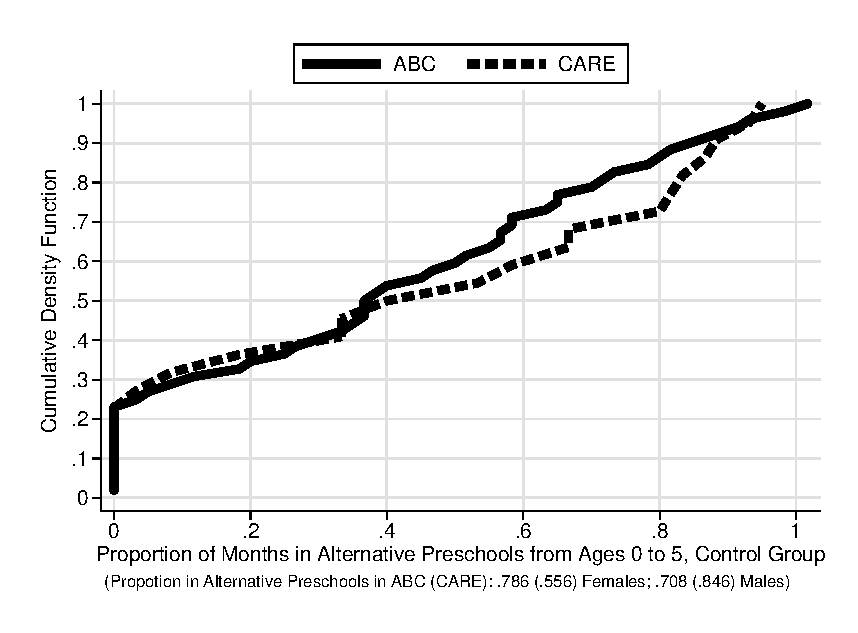
\includegraphics[width=20em]{output/abccare_controlcontamination.eps}
\end{figure}
\hyperlink{abc_subsidized}{\beamergotobutton{Proportion Subsidized, ABC}}
\hyperlink{care_subsidized}{\beamergotobutton{Proportion Subsidized, CARE}}
\end{frame}

%% ---------------------------------------------------------------------------

\begin{frame}
\frametitle{Alternative Preschools Take-up, ABC}\label{abc_subsidized}
\begin{figure}
\caption{Average Months in Control Substitution, ABC}
	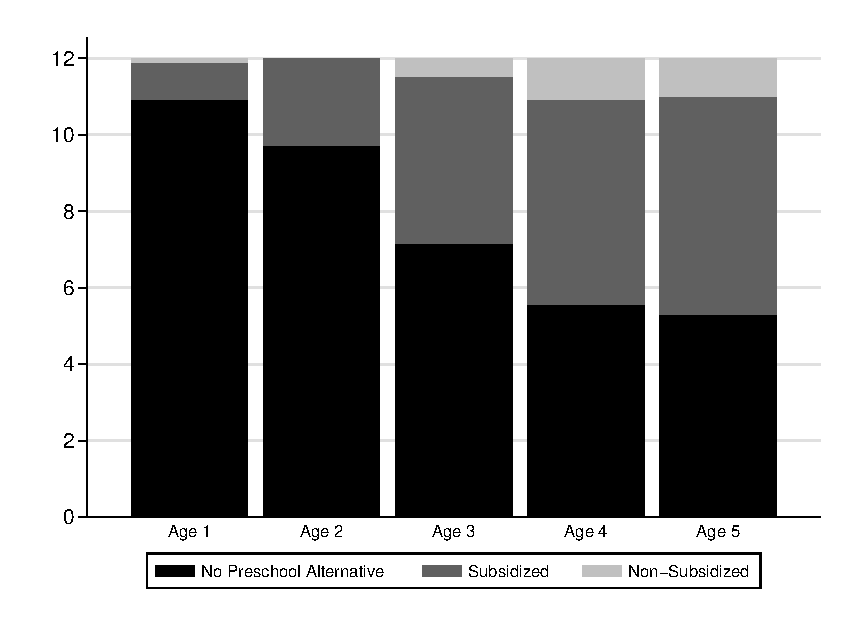
\includegraphics[width=18em]{output/blackwhite_CCnumber}
\end{figure}
\hyperlink{substitution}{\beamerreturnbutton{Back}}
\end{frame}

%% ---------------------------------------------------------------------------

\begin{frame}
\frametitle{Alternative Preschools Take-up, CARE}\label{care_subsidized}
\begin{figure}
\caption{Average Months in Control Substitution, CARE}
	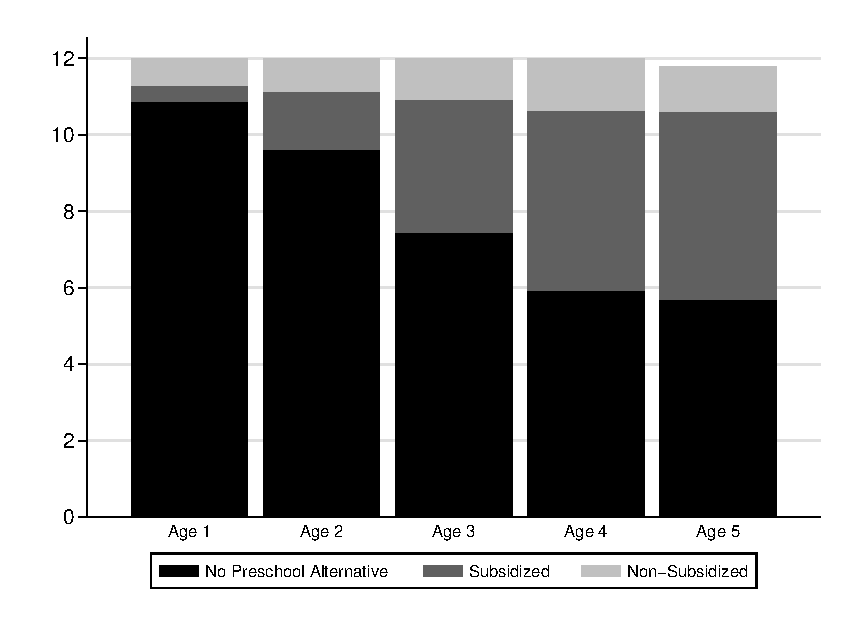
\includegraphics[width=18em]{output/blackwhite_CCnumber_care}
\end{figure}
\hyperlink{substitution}{\beamerreturnbutton{Back}}
\end{frame}

%% ---------------------------------------------------------------------------

\begin{frame}
\frametitle{Treatment Effects before Control Substitution, Females}
\begin{center}
\begin{table}
	\caption{Treatment Effects, Females} \label{tab:onsetsfemales}
	\scalebox{.60}{

 \begin{tabular}{cccc}
  \toprule
      \scriptsize{Variable} & \scriptsize{Age} & \scriptsize{(1)} & \scriptsize{(2)} \\ 
    \midrule  

  \mc{1}{l}{\scriptsize{Std. IQ Test}} & \mc{1}{c}{\scriptsize{2}} & \mc{1}{c}{\scriptsize{10.700}} & \mc{1}{c}{\scriptsize{9.200}} \\  

     &  & \mc{1}{c}{\scriptsize{\textbf{(0.000)}}} & \mc{1}{c}{\scriptsize{\textbf{(0.000)}}} \\  

     & \mc{1}{c}{\scriptsize{3}} & \mc{1}{c}{\scriptsize{13.333}} & \mc{1}{c}{\scriptsize{12.563}} \\  

     &  & \mc{1}{c}{\scriptsize{\textbf{(0.000)}}} & \mc{1}{c}{\scriptsize{\textbf{(0.000)}}}  \\ 
     \midrule
         \mc{1}{l}{\scriptsize{HOME Score}} & \mc{1}{c}{\scriptsize{0.5}} & \mc{1}{c}{\scriptsize{1.581}} & \mc{1}{c}{\scriptsize{0.749}}  \\  

     &  & \mc{1}{c}{\scriptsize{\textbf{(0.039)}}} & \mc{1}{c}{\scriptsize{(0.250)}}  \\  

     & \mc{1}{c}{\scriptsize{1.5}} & \mc{1}{c}{\scriptsize{2.668}} & \mc{1}{c}{\scriptsize{1.723}} \\  

     &  & \mc{1}{c}{\scriptsize{\textbf{(0.013)}}} & \mc{1}{c}{\scriptsize{(0.158)}} \\  

     & \mc{1}{c}{\scriptsize{2.5}} & \mc{1}{c}{\scriptsize{0.762}} & \mc{1}{c}{\scriptsize{0.832}} \\  

     &  & \mc{1}{c}{\scriptsize{(0.224)}} & \mc{1}{c}{\scriptsize{(0.237)}}  \\ 
     \midrule  
      \mc{1}{l}{\scriptsize{Parental Income}} & \mc{1}{c}{\scriptsize{1.5}} & \mc{1}{c}{\scriptsize{4,516}} & \mc{1}{c}{\scriptsize{7,539}} \\  

     &  & \mc{1}{c}{\scriptsize{\textbf{(0.066)}}} & \mc{1}{c}{\scriptsize{\textbf{(0.013)}}} \\  

     & \mc{1}{c}{\scriptsize{2.5}} & \mc{1}{c}{\scriptsize{222}} & \mc{1}{c}{\scriptsize{400}}  \\  

     &  & \mc{1}{c}{\scriptsize{(0.474)}} & \mc{1}{c}{\scriptsize{(0.434)}} \\  
     \midrule
      \mc{1}{l}{\scriptsize{Mother Works}} & \mc{1}{c}{\scriptsize{2}} & \mc{1}{c}{\scriptsize{0.168}} & \mc{1}{c}{\scriptsize{0.124}} \\  

     &  & \mc{1}{c}{\scriptsize{\textbf{(0.026)}}} & \mc{1}{c}{\scriptsize{\textbf{(0.079)}}} \\  

     & \mc{1}{c}{\scriptsize{3}} & \mc{1}{c}{\scriptsize{0.087}} & \mc{1}{c}{\scriptsize{0.047}}  \\  

     &  & \mc{1}{c}{\scriptsize{(0.237)}} & \mc{1}{c}{\scriptsize{(0.368)}}  \\  
     \bottomrule
     \end{tabular}
}
\end{table}
\end{center}
\end{frame}

%% ---------------------------------------------------------------------------

\begin{frame}
\frametitle{Treatment Effects before Control Substitution, Males}
\begin{center}
\begin{table}
	\caption{Treatment Effects, Males} \label{tab:onsetsmales}
	\scalebox{.60}{\begin{table}[htbp]
\begin{center}
\caption{Results from Ages 0 to 3: Males}
 \begin{tabular}{cccccccccc}
  \toprule
      \scriptsize{Variable} & \scriptsize{Age} & \scriptsize{(1)} & \scriptsize{(2)} & \scriptsize{(3)} & \scriptsize{(4)} & \scriptsize{(5)} & \scriptsize{(6)} & \scriptsize{(7)} & \scriptsize{(8)} \\ 
    \midrule  

\mc{1}{l}{\scriptsize{Std. IQ Test}} & \mc{1}{c}{\scriptsize{2}} & \mc{1}{c}{\scriptsize{9.528}} & \mc{1}{c}{\scriptsize{11.036}} & \mc{1}{c}{\scriptsize{6.875}} & \mc{1}{c}{\scriptsize{10.704}} & \mc{1}{c}{\scriptsize{7.944}} & \mc{1}{c}{\scriptsize{10.286}} & \mc{1}{c}{\scriptsize{11.497}} & \mc{1}{c}{\scriptsize{11.080}} \\  

     &  & \mc{1}{c}{\scriptsize{\textbf{(0.000)}}} & \mc{1}{c}{\scriptsize{\textbf{(0.000)}}} & \mc{1}{c}{\scriptsize{\textbf{(0.026)}}} & \mc{1}{c}{\scriptsize{\textbf{(0.026)}}} & \mc{1}{c}{\scriptsize{\textbf{(0.013)}}} & \mc{1}{c}{\scriptsize{\textbf{(0.000)}}} & \mc{1}{c}{\scriptsize{\textbf{(0.000)}}} & \mc{1}{c}{\scriptsize{\textbf{(0.000)}}} \\  

     & \mc{1}{c}{\scriptsize{3}} & \mc{1}{c}{\scriptsize{13.410}} & \mc{1}{c}{\scriptsize{14.873}} & \mc{1}{c}{\scriptsize{13.896}} & \mc{1}{c}{\scriptsize{17.254}} & \mc{1}{c}{\scriptsize{15.474}} & \mc{1}{c}{\scriptsize{13.271}} & \mc{1}{c}{\scriptsize{14.229}} & \mc{1}{c}{\scriptsize{14.302}} \\  

     &  & \mc{1}{c}{\scriptsize{\textbf{(0.000)}}} & \mc{1}{c}{\scriptsize{\textbf{(0.000)}}} & \mc{1}{c}{\scriptsize{\textbf{(0.000)}}} & \mc{1}{c}{\scriptsize{\textbf{(0.000)}}} & \mc{1}{c}{\scriptsize{\textbf{(0.000)}}} & \mc{1}{c}{\scriptsize{\textbf{(0.000)}}} & \mc{1}{c}{\scriptsize{\textbf{(0.000)}}} & \mc{1}{c}{\scriptsize{\textbf{(0.000)}}} \\  
     \midrule
         \mc{1}{l}{\scriptsize{HOME Score}} & \mc{1}{c}{\scriptsize{0.5}} & \mc{1}{c}{\scriptsize{0.372}} & \mc{1}{c}{\scriptsize{0.039}} & \mc{1}{c}{\scriptsize{0.944}} & \mc{1}{c}{\scriptsize{-0.416}} & \mc{1}{c}{\scriptsize{0.431}} & \mc{1}{c}{\scriptsize{0.143}} & \mc{1}{c}{\scriptsize{0.069}} & \mc{1}{c}{\scriptsize{-0.080}} \\  

     &  & \mc{1}{c}{\scriptsize{(0.316)}} & \mc{1}{c}{\scriptsize{(0.487)}} & \mc{1}{c}{\scriptsize{(0.316)}} & \mc{1}{c}{\scriptsize{(0.618)}} & \mc{1}{c}{\scriptsize{(0.421)}} & \mc{1}{c}{\scriptsize{(0.447)}} & \mc{1}{c}{\scriptsize{(0.474)}} & \mc{1}{c}{\scriptsize{(0.487)}} \\  

     & \mc{1}{c}{\scriptsize{1.5}} & \mc{1}{c}{\scriptsize{-0.500}} & \mc{1}{c}{\scriptsize{-0.874}} & \mc{1}{c}{\scriptsize{0.431}} & \mc{1}{c}{\scriptsize{-1.123}} & \mc{1}{c}{\scriptsize{0.216}} & \mc{1}{c}{\scriptsize{-0.766}} & \mc{1}{c}{\scriptsize{-0.865}} & \mc{1}{c}{\scriptsize{-0.872}} \\  

     &  & \mc{1}{c}{\scriptsize{(0.645)}} & \mc{1}{c}{\scriptsize{(0.750)}} & \mc{1}{c}{\scriptsize{(0.447)}} & \mc{1}{c}{\scriptsize{(0.684)}} & \mc{1}{c}{\scriptsize{(0.447)}} & \mc{1}{c}{\scriptsize{(0.711)}} & \mc{1}{c}{\scriptsize{(0.737)}} & \mc{1}{c}{\scriptsize{(0.724)}} \\  

     & \mc{1}{c}{\scriptsize{2.5}} & \mc{1}{c}{\scriptsize{0.141}} & \mc{1}{c}{\scriptsize{0.886}} & \mc{1}{c}{\scriptsize{1.654}} & \mc{1}{c}{\scriptsize{3.806}} & \mc{1}{c}{\scriptsize{2.232}} & \mc{1}{c}{\scriptsize{-0.292}} & \mc{1}{c}{\scriptsize{0.543}} & \mc{1}{c}{\scriptsize{0.145}} \\  

     &  & \mc{1}{c}{\scriptsize{(0.474)}} & \mc{1}{c}{\scriptsize{(0.263)}} & \mc{1}{c}{\scriptsize{(0.197)}} & \mc{1}{c}{\scriptsize{(0.105)}} & \mc{1}{c}{\scriptsize{(0.145)}} & \mc{1}{c}{\scriptsize{(0.618)}} & \mc{1}{c}{\scriptsize{(0.395)}} & \mc{1}{c}{\scriptsize{(0.487)}} \\  
	\midrule
	 \mc{1}{l}{\scriptsize{Parental Income}} & \mc{1}{c}{\scriptsize{1.5}} & \mc{1}{c}{\scriptsize{330}} & \mc{1}{c}{\scriptsize{-97.199}} & \mc{1}{c}{\scriptsize{-1,046}} & \mc{1}{c}{\scriptsize{-2,384}} & \mc{1}{c}{\scriptsize{-1,168}} & \mc{1}{c}{\scriptsize{-9.245}} & \mc{1}{c}{\scriptsize{-26.663}} & \mc{1}{c}{\scriptsize{872}} \\  

     &  & \mc{1}{c}{\scriptsize{(0.408)}} & \mc{1}{c}{\scriptsize{(0.461)}} & \mc{1}{c}{\scriptsize{(0.579)}} & \mc{1}{c}{\scriptsize{(0.645)}} & \mc{1}{c}{\scriptsize{(0.632)}} & \mc{1}{c}{\scriptsize{(0.434)}} & \mc{1}{c}{\scriptsize{(0.487)}} & \mc{1}{c}{\scriptsize{(0.329)}} \\  

     & \mc{1}{c}{\scriptsize{2.5}} & \mc{1}{c}{\scriptsize{673}} & \mc{1}{c}{\scriptsize{-941}} & \mc{1}{c}{\scriptsize{-1,167}} & \mc{1}{c}{\scriptsize{-3,542}} & \mc{1}{c}{\scriptsize{-1,858}} & \mc{1}{c}{\scriptsize{478}} & \mc{1}{c}{\scriptsize{-839}} & \mc{1}{c}{\scriptsize{232}} \\  

     &  & \mc{1}{c}{\scriptsize{(0.382)}} & \mc{1}{c}{\scriptsize{(0.645)}} & \mc{1}{c}{\scriptsize{(0.618)}} & \mc{1}{c}{\scriptsize{(0.750)}} & \mc{1}{c}{\scriptsize{(0.671)}} & \mc{1}{c}{\scriptsize{(0.408)}} & \mc{1}{c}{\scriptsize{(0.605)}} & \mc{1}{c}{\scriptsize{(0.513)}} \\  
     \midrule
      \mc{1}{l}{\scriptsize{Mother Works}} & \mc{1}{c}{\scriptsize{2}} & \mc{1}{c}{\scriptsize{0.056}} & \mc{1}{c}{\scriptsize{0.038}} & \mc{1}{c}{\scriptsize{0.264}} & \mc{1}{c}{\scriptsize{0.184}} & \mc{1}{c}{\scriptsize{0.240}} & \mc{1}{c}{\scriptsize{-0.004}} & \mc{1}{c}{\scriptsize{0.008}} & \mc{1}{c}{\scriptsize{-0.018}} \\  

     &  & \mc{1}{c}{\scriptsize{(0.289)}} & \mc{1}{c}{\scriptsize{(0.368)}} & \mc{1}{c}{\scriptsize{\textbf{(0.066)}}} & \mc{1}{c}{\scriptsize{(0.145)}} & \mc{1}{c}{\scriptsize{\textbf{(0.079)}}} & \mc{1}{c}{\scriptsize{(0.447)}} & \mc{1}{c}{\scriptsize{(0.487)}} & \mc{1}{c}{\scriptsize{(0.539)}} \\  

     & \mc{1}{c}{\scriptsize{3}} & \mc{1}{c}{\scriptsize{0.150}} & \mc{1}{c}{\scriptsize{0.125}} & \mc{1}{c}{\scriptsize{0.261}} & \mc{1}{c}{\scriptsize{0.184}} & \mc{1}{c}{\scriptsize{0.240}} & \mc{1}{c}{\scriptsize{0.117}} & \mc{1}{c}{\scriptsize{0.117}} & \mc{1}{c}{\scriptsize{0.117}} \\  

     &  & \mc{1}{c}{\scriptsize{\textbf{(0.066)}}} & \mc{1}{c}{\scriptsize{(0.184)}} & \mc{1}{c}{\scriptsize{\textbf{(0.079)}}} & \mc{1}{c}{\scriptsize{(0.145)}} & \mc{1}{c}{\scriptsize{\textbf{(0.079)}}} & \mc{1}{c}{\scriptsize{(0.158)}} & \mc{1}{c}{\scriptsize{(0.197)}} & \mc{1}{c}{\scriptsize{(0.171)}} \\ 
     \bottomrule
     \end{tabular}}
\end{table}
\end{center}
\end{frame}

%% ---------------------------------------------------------------------------

\begin{frame}[shrink=30]
\frametitle{Comparison of the Estimates}
\begin{tabular}{llcccccc}
											   && \multicolumn{2}{c}{Yale}&\multicolumn{2}{c}{Tuesday}&\multicolumn{2}{c}{Current}	\\
		&										& IRR	& B/C	& IRR	& B/C	& IRR	& B/C			\\
		& Baseline								& 0.05 	& 1.56	& 0.10	& 2.30	& 0.11	& 3.52			\\
		&										& (0.12)& (1.42)& (0.12)& (1.56)& (0.12)& (2.67)		\\
Females & Relative to Staying at Home			& 	.	& 	.	&-0.14&\textbf{4.97}		& -0.14	& \textbf{4.95}	\\
		&										&	.	&	.	&(0.13)	&(2.02)	& (0.13)& (2.02)		\\
		& Relative to Alternative Preschools	&   .	&   .	&0.08	&1.58		& 0.09	& 2.88			\\
		&										&	.	&	.	&(0.14)	&(1.20)	& (0.11)& (1.85)		\\ \hline
		& Baseline								& \textbf{0.25} & 6.91	& 0.15&7.88& \textbf{0.16}	& 9.21	\\
		&										& (0.10)& 4.43	& (0.13)&(8.06)	& (0.11)& (8.33)		\\ 
Males 	& Relative to Staying at Home			& 	.	& 	.	&0.02	&0.55	& 0.06	& 4.29 			\\
		&										&	.	&	.	&(0.13)&(3.00)& (0.11)& (4.75) 		\\ 
		& Relative to Alternative Preschools	& .	& .	&\textbf{0.20}&\textbf{12.24}& \textbf{0.21}& \textbf{13.64}\\
		&										&	.	&	.	&(0.14)		&(5.39)		& (0.13)& (5.72)			\\ \hline
		& Baseline						& \textbf{0.16} & \textbf{4.30}& \textbf{0.13}&4.35 & \textbf{0.13}	& \textbf{5.80} \\
		&										& (0.06)&(2.15)	&(0.11)&(2.57)& (0.06)& (2.86) 			\\ 
Pooled  & Relative to Staying at Home			& 	.	& 	.	&\textbf{0.09}&3.78		& \textbf{0.10}	& 5.18  		\\
		&										&	.	&	.	&(0.05)&(2.15)& (0.05)& (3.19) 			\\ 
		& Relative to Alternative Preschools	& 	.	& 	.	&\textbf{0.12}&4.34& \textbf{0.13}	& \textbf{5.56} 		\\
		&										&	.	&	.	&(0.09)&(2.67)& (0.06)	& (2.88) 			\\ 
\end{tabular}
\end{frame}

%% ---------------------------------------------------------------------------

\begin{frame}
\frametitle{Current Estimates}
\begin{center}
\begin{table}
	\caption{CBA Summary}
	\scalebox{.40}{\begin{tabular}{l r r r r r r r r r}																			
\toprule																			
&       \mc{3}{c}{Females}      &       \mc{3}{c}{Males}        &       \mc{3}{c}{Pooled}       \\																			
\cmidrule(lr){2-4}      \cmidrule(lr){5-7}      \cmidrule(lr){8-10}																			
Removed Component       &       NPV     &       IRR     &       B/C     &       NPV     &       IRR     &       B/C     &       NPV     &       IRR     &       B/C     \\																			
\midrule																			
None	&	161,759	&	\textbf{10.1\%}	&	\textbf{2.61}	&	919,049	&	\textbf{14.7\%}	&	\textbf{10.19}	&	636,674	&	\textbf{13.7\%}	&	\textbf{7.33}	\\
	&		&	(6\%)	&	(0.73)	&		&	(4\%)	&	(2.93)	&		&	(3\%)	&	(1.84)	\\ \\
Parental Income	&	148,854	&	4\%	&	1.12	&	107,907	&	\textbf{11\%}	&	\textbf{9.10}	&	116,953	&	\textbf{9\%}	&	\textbf{6.17}	\\
	&		&	(2\%)	&	(0.65)	&		&	(3\%)	&	(2.92)	&		&	(3\%)	&	(1.87)	\\
Subject Labor Income	&	41,908	&	9\%	&	\textbf{2.21}	&	238,105	&	\textbf{13\%}	&	\textbf{7.75}	&	133,032	&	\textbf{13\%}	&	\textbf{6.03}	\\
	&		&	(6\%)	&	(0.66)	&		&	(5\%)	&	(2.23)	&		&	(4\%)	&	(1.77)	\\
Subject Transfer Income	&	419	&	\textbf{10\%}	&	\textbf{2.61}	&	-7,265	&	\textbf{15\%}	&	\textbf{10.26}	&	-4,372	&	\textbf{14\%}	&	\textbf{7.38}	\\
	&		&	(6\%)	&	(0.73)	&		&	(4\%)	&	(2.93)	&		&	(3\%)	&	(1.84)	\\
Subject QALY	&	42,102	&	9\%	&	\textbf{2.20}	&	106,218	&	\textbf{14\%}	&	\textbf{9.14}	&	87,181	&	\textbf{13\%}	&	\textbf{6.48}	\\
	&		&	(6\%)	&	(0.69)	&		&	(6\%)	&	(2.73)	&		&	(5\%)	&	(1.79)	\\
Medical Expenditures	&	-16,037	&	9\%	&	\textbf{2.77}	&	-42,038	&	\textbf{15\%}	&	\textbf{10.61}	&	-31,221	&	\textbf{14\%}	&	\textbf{7.65}	\\
	&		&	(6\%)	&	(0.76)	&		&	(3\%)	&	(2.89)	&		&	(3\%)	&	(1.85)	\\
Alternative Preschools	&	16,691	&	8\%	&	\textbf{2.45}	&	13,434	&	\textbf{14\%}	&	\textbf{10.05}	&	14,659	&	\textbf{12\%}	&	\textbf{7.19}	\\
	&		&	(5\%)	&	(0.73)	&		&	(4\%)	&	(2.92)	&		&	(3\%)	&	(1.84)	\\
Education Costs	&	1,457	&	\textbf{10\%}	&	\textbf{2.59}	&	-7,852	&	\textbf{15\%}	&	\textbf{10.26}	&	-4,518	&	\textbf{14\%}	&	\textbf{7.37}	\\
	&		&	(6\%)	&	(0.72)	&		&	(4\%)	&	(2.93)	&		&	(3\%)	&	(1.86)	\\
Crime Costs	&	31,668	&	10\%	&	\textbf{2.34}	&	638,923	&	\textbf{9\%}	&	4.08	&	450,368	&	\textbf{8\%}	&	\textbf{3.06}	\\
	&		&	(6\%)	&	(0.62)	&		&	(5\%)	&	(2.18)	&	&	(4\%)	&	(1.01)	\\ \\
Deadweight Loss	&		&	\textbf{18\%}	&	\textbf{3.83}	&		&	\textbf{19\%}	&	\textbf{15.38}	&		&	\textbf{18\%}	&	\textbf{11.01}	\\
	&		&	(12\%)	&	(1.04)	&		&	(6\%)	&	(4.35)	&		&	(5\%)	&	(2.79)	\\
0\% Discount Rate	&		&		&	\textbf{5.06}	&		&		&	\textbf{25.45}	&		&		&	\textbf{17.40}	\\
	&		&		&	(2.82)	&		&		&	(10.42)	&		&		&	(5.90)	\\
7\% Discount Rate	&		&		&	\textbf{1.49}	&		&		&	\textbf{3.78}	&		&		&	\textbf{2.91}	\\
	&		&		&	(0.32)	&		&		&	(0.79)	&		&		&	(0.59)	\\
\bottomrule																			
\end{tabular}																			
}
\end{table}
\end{center}
\end{frame}

%% ---------------------------------------------------------------------------

\begin{frame}
\frametitle{IRR Females, Treatment vs. Control} 
\begin{figure}
	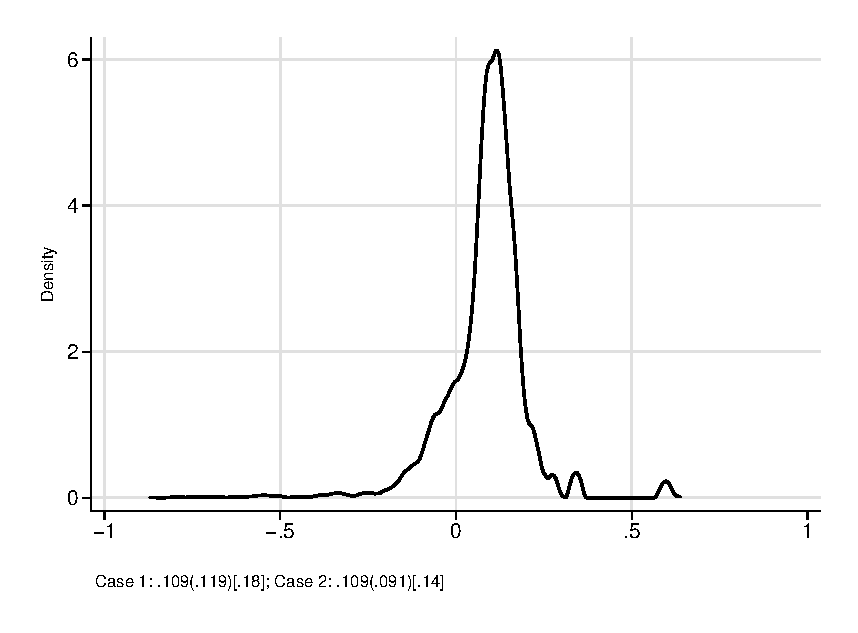
\includegraphics[width=.8\columnwidth]{output/irr_2_sexf.eps}
\end{figure}
\end{frame}

%% ---------------------------------------------------------------------------

\begin{frame}
\frametitle{IRR Males, Treatment vs. Control} 
\begin{figure}
	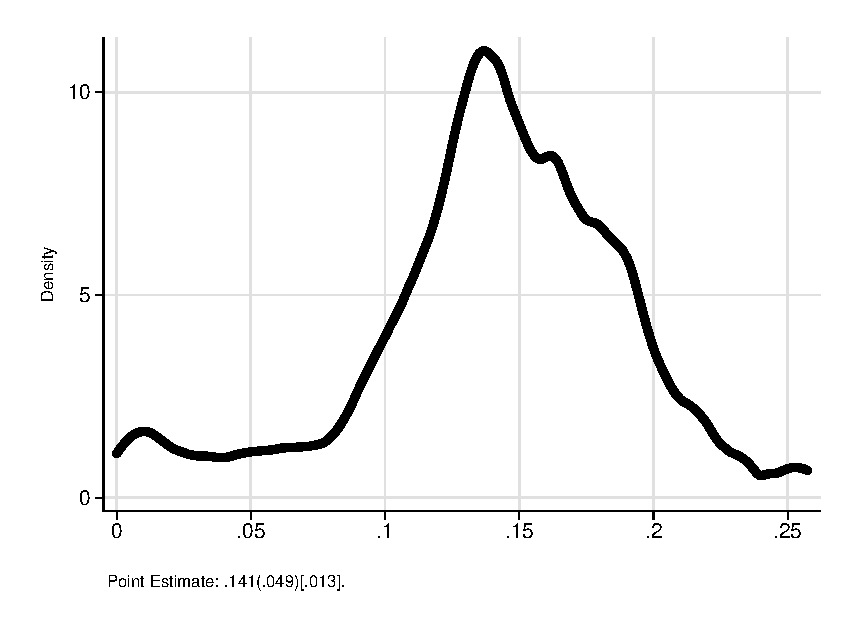
\includegraphics[width=.8\columnwidth]{output/irr_2_sexm.eps}
\end{figure}
\end{frame}

%% ---------------------------------------------------------------------------

\begin{frame}
\frametitle{IRR Pooled, Treatment vs. Control} 
\begin{figure}
	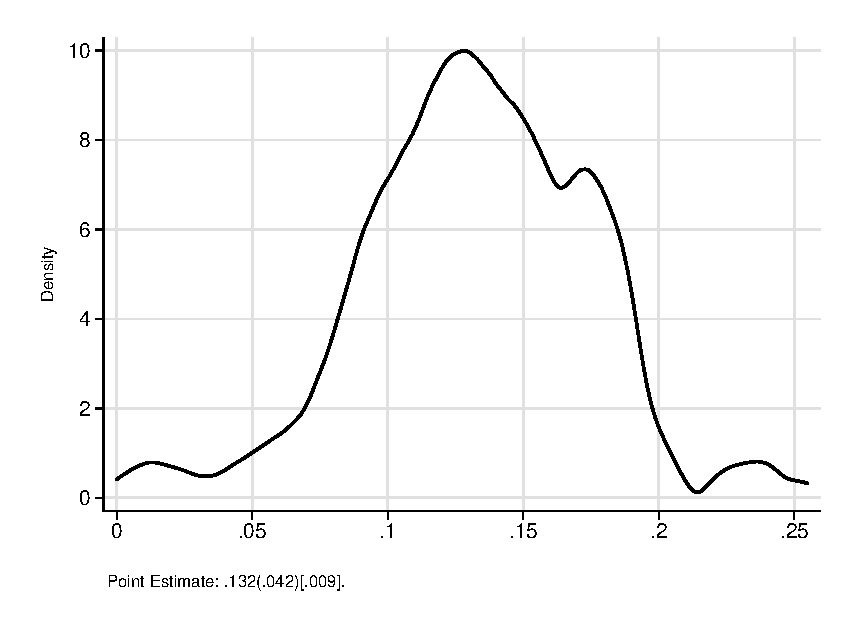
\includegraphics[width=.8\columnwidth]{output/irr_2_sexp.eps}
\end{figure}
\end{frame}

%% ---------------------------------------------------------------------------

\begin{frame}
\frametitle{IRR Females, Treatment vs. Control (Stay at Home)} 
\begin{figure}
	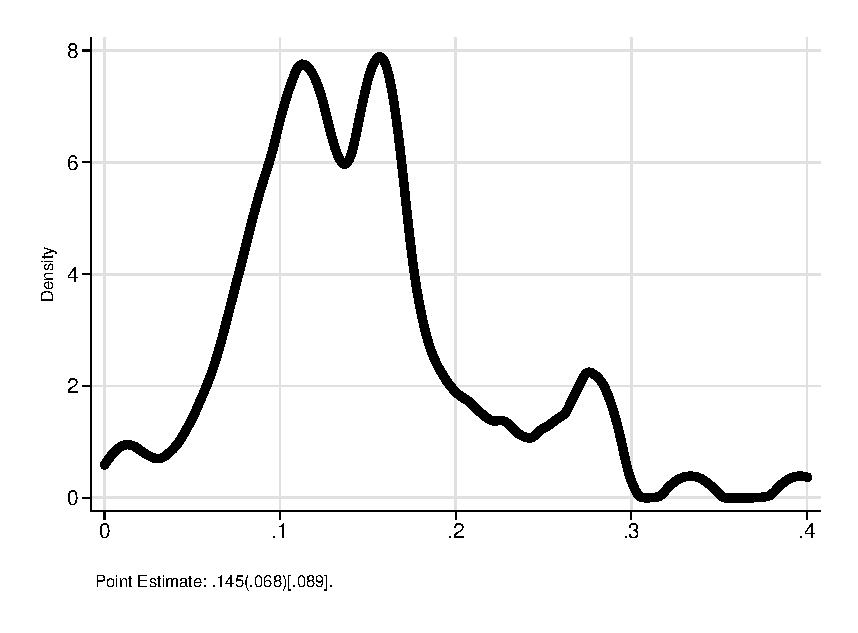
\includegraphics[width=.8\columnwidth]{output/irr_5_sexf.eps}
\end{figure}
\end{frame}

%% ---------------------------------------------------------------------------

\begin{frame}
\frametitle{IRR Males, Treatment vs. Control (Stay at Home)} 
\begin{figure}
	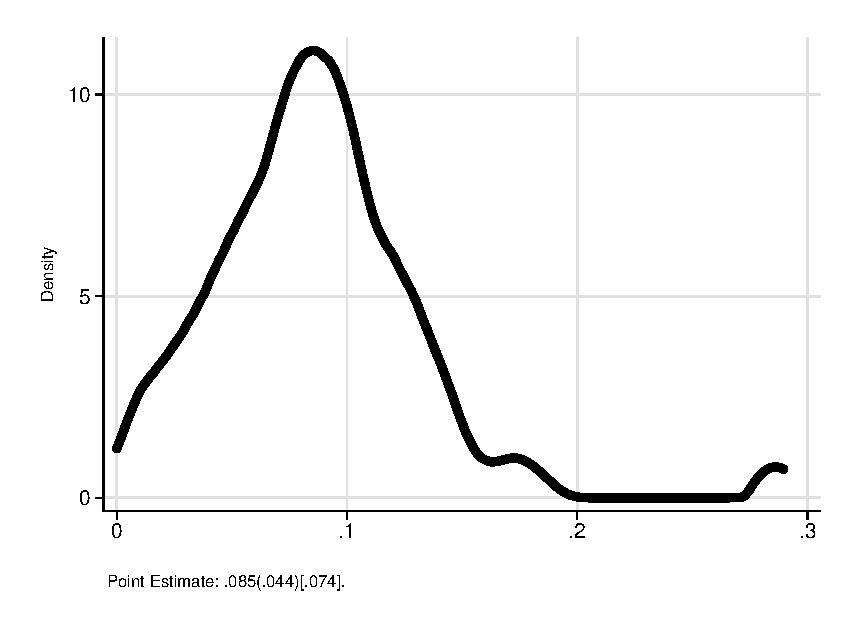
\includegraphics[width=.8\columnwidth]{output/irr_5_sexm.eps}
\end{figure}
\end{frame}

%% ---------------------------------------------------------------------------

\begin{frame}
\frametitle{IRR Pooled, Treatment vs. Control (Stay at Home)} 
\begin{figure}
	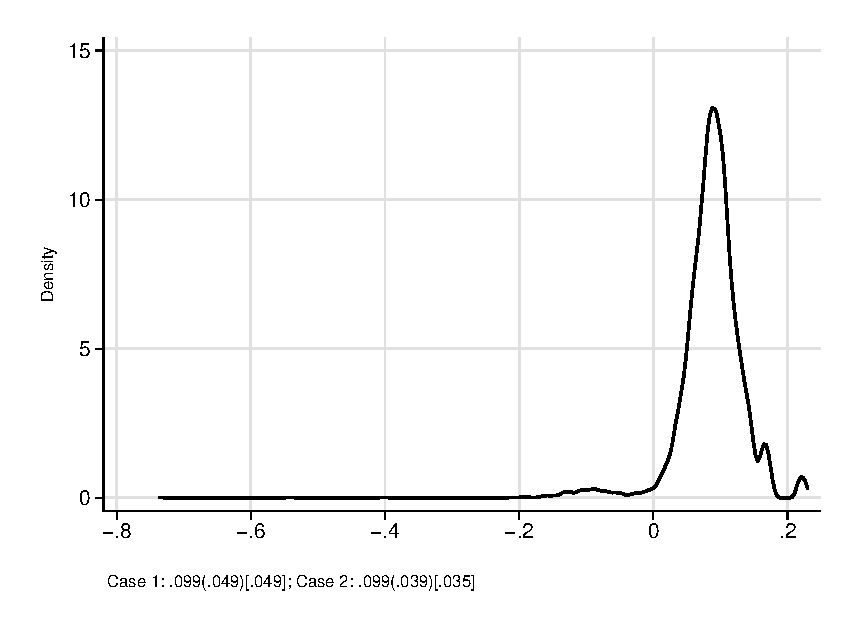
\includegraphics[width=.8\columnwidth]{output/irr_5_sexp.eps}
\end{figure}
\end{frame}

%% ---------------------------------------------------------------------------

\begin{frame}
\frametitle{IRR Females, Treatment vs. Control (Alternative Preschools)} 
\begin{figure}
	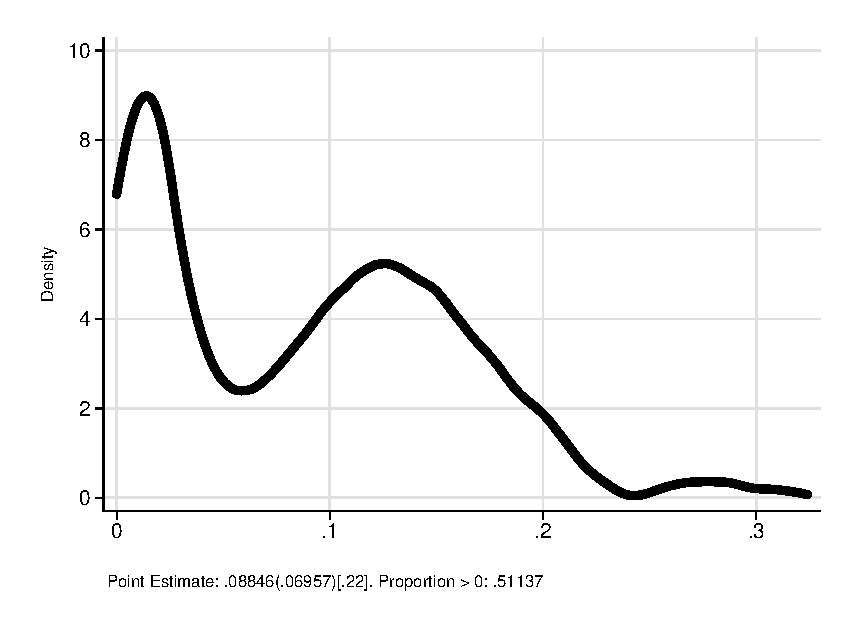
\includegraphics[width=.8\columnwidth]{output/irr_8_sexf.eps}
\end{figure}
\end{frame}

%% ---------------------------------------------------------------------------

\begin{frame}
\frametitle{IRR Males, Treatment vs. Control (Alternative Preschools)} 
\begin{figure}
	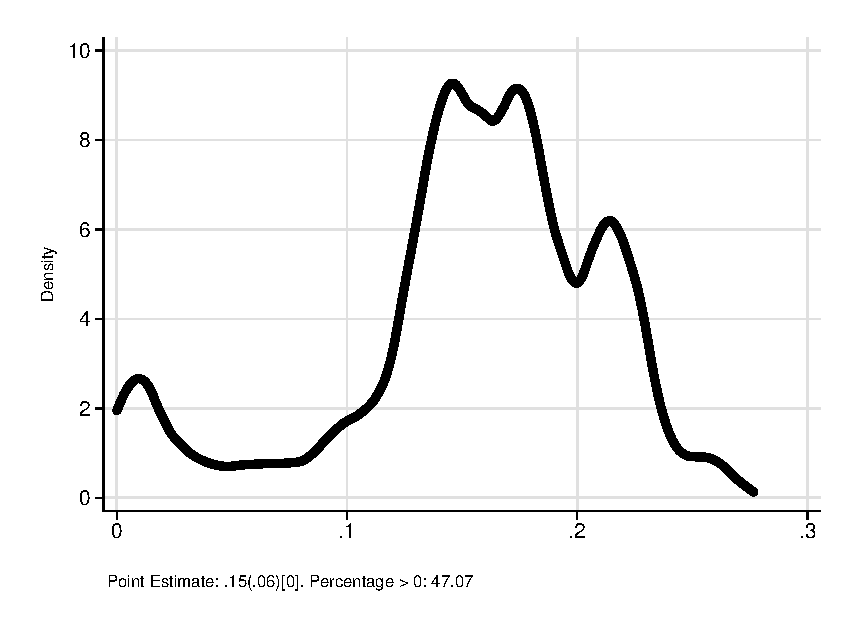
\includegraphics[width=.8\columnwidth]{output/irr_8_sexm.eps}
\end{figure}
\end{frame}

%% ---------------------------------------------------------------------------

\begin{frame}
\frametitle{IRR Pooled, Treatment vs. Control (Alternative Preschools)} 
\begin{figure}
	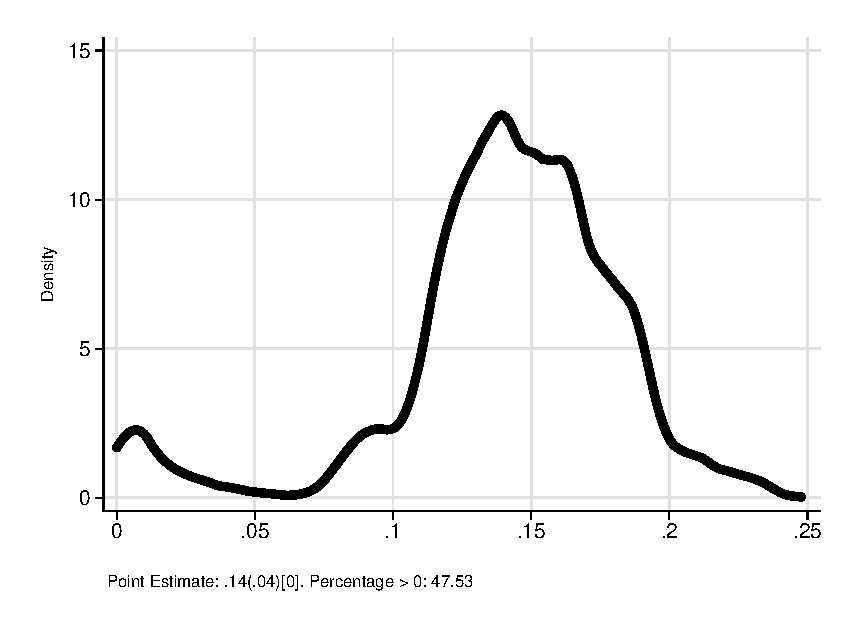
\includegraphics[width=.8\columnwidth]{output/irr_8_sexp.eps}
\end{figure}
\end{frame}

%% ---------------------------------------------------------------------------

\begin{frame}
\frametitle{B/C Females, Treatment vs. Control} 
\begin{figure}
	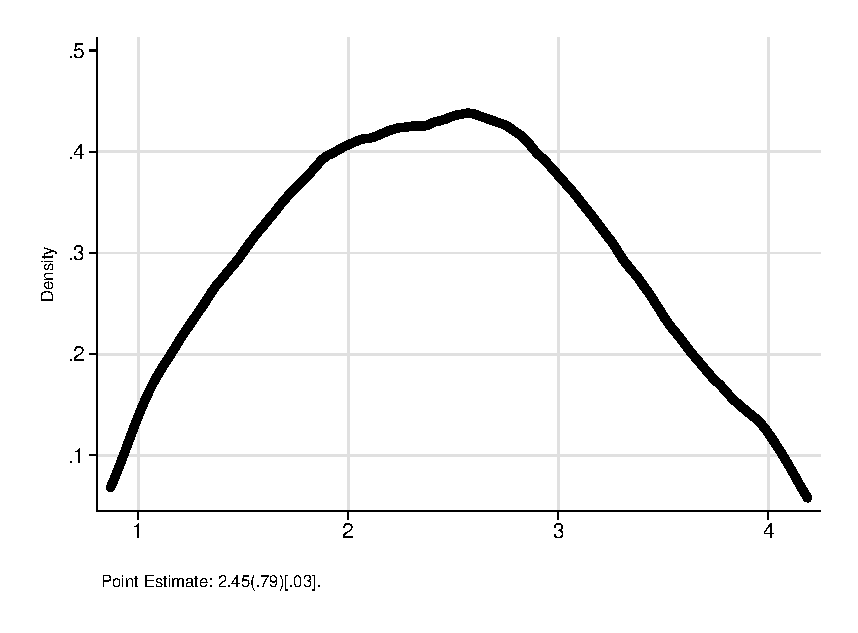
\includegraphics[width=.8\columnwidth]{output/ratios_2_sexf.eps}
\end{figure}
\end{frame}

%% ---------------------------------------------------------------------------

\begin{frame}
\frametitle{B/C Males, Treatment vs. Control} 
\begin{figure}
	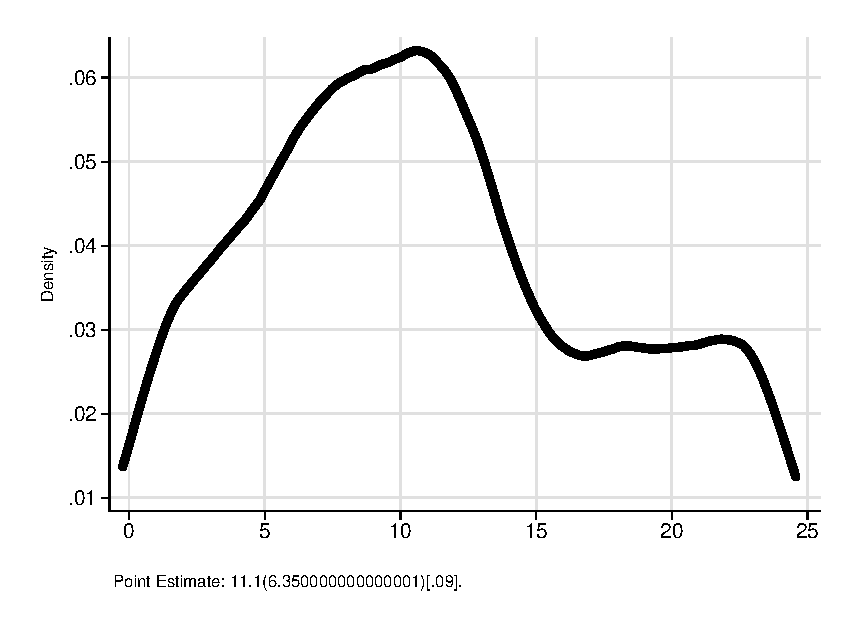
\includegraphics[width=.8\columnwidth]{output/ratios_2_sexm.eps}
\end{figure}
\end{frame}

%% ---------------------------------------------------------------------------

\begin{frame}
\frametitle{B/C Pooled, Treatment vs. Control} 
\begin{figure}
	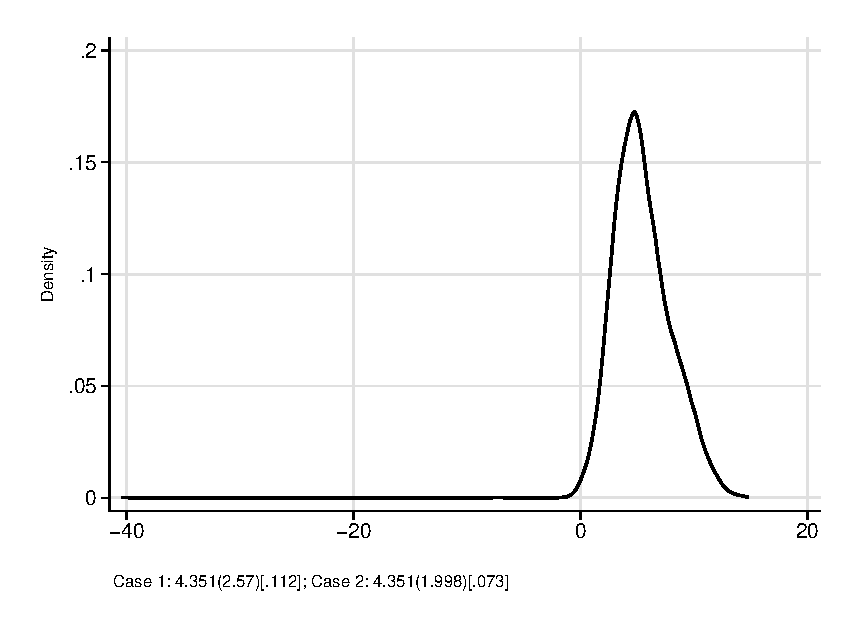
\includegraphics[width=.8\columnwidth]{output/ratios_2_sexp.eps}
\end{figure}
\end{frame}

%% ---------------------------------------------------------------------------

\begin{frame}
\frametitle{B/C Females, Treatment vs. Control (Stay at Home)} 
\begin{figure}
	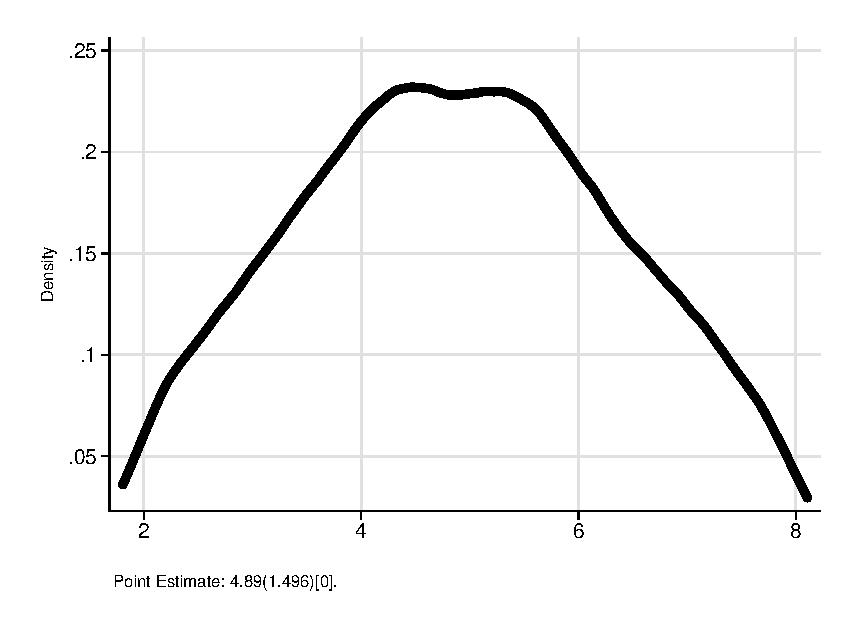
\includegraphics[width=.8\columnwidth]{output/ratios_5_sexf.eps}
\end{figure}
\end{frame}

%% ---------------------------------------------------------------------------

\begin{frame}
\frametitle{B/C Males, Treatment vs. Control (Stay at Home)} 
\begin{figure}
	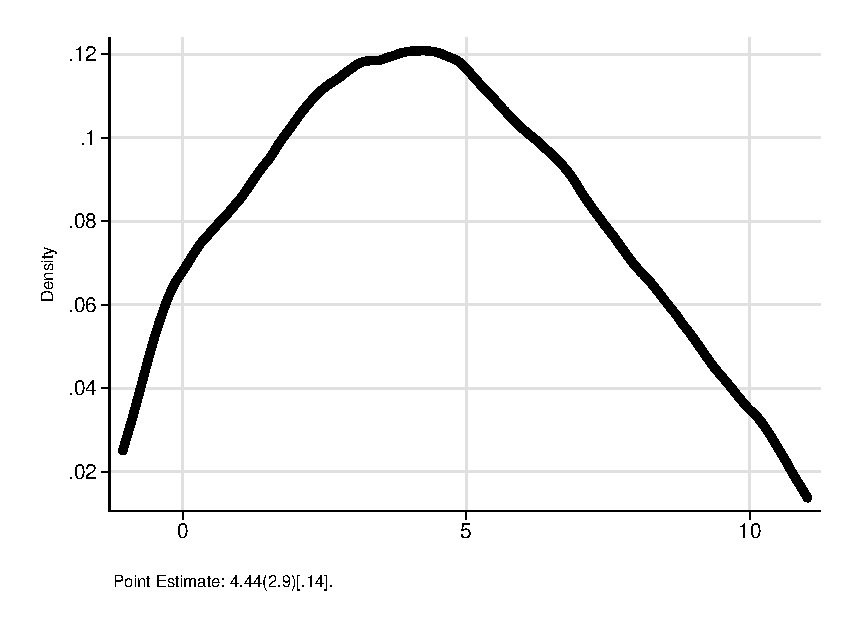
\includegraphics[width=.8\columnwidth]{output/ratios_5_sexm.eps}
\end{figure}
\end{frame}

%% ---------------------------------------------------------------------------

\begin{frame}
\frametitle{B/C Pooled, Treatment vs. Control (Stay at Home)} 
\begin{figure}
	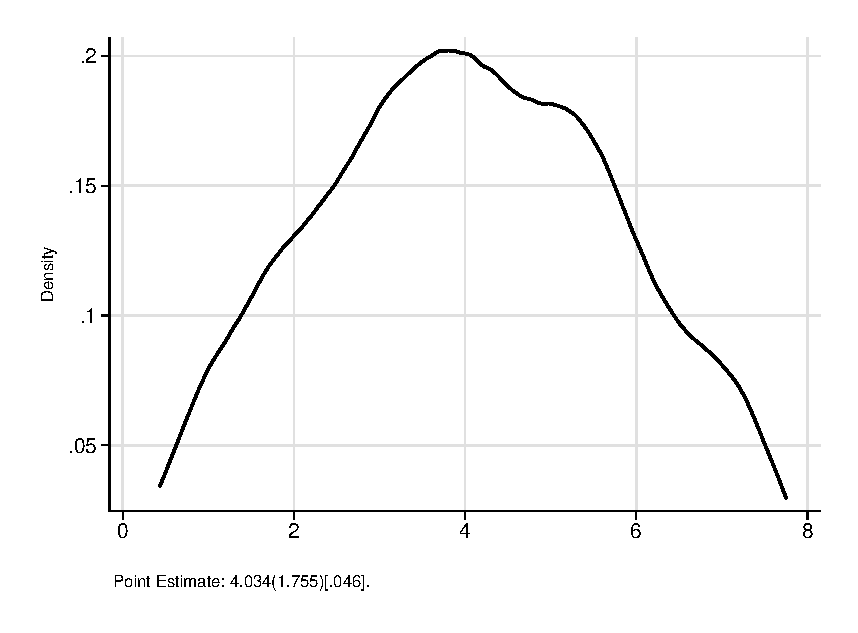
\includegraphics[width=.8\columnwidth]{output/ratios_5_sexp.eps}
\end{figure}
\end{frame}

%% ---------------------------------------------------------------------------

\begin{frame}
\frametitle{B/C Females, Treatment vs. Control (Alternative Preschools)} 
\begin{figure}
	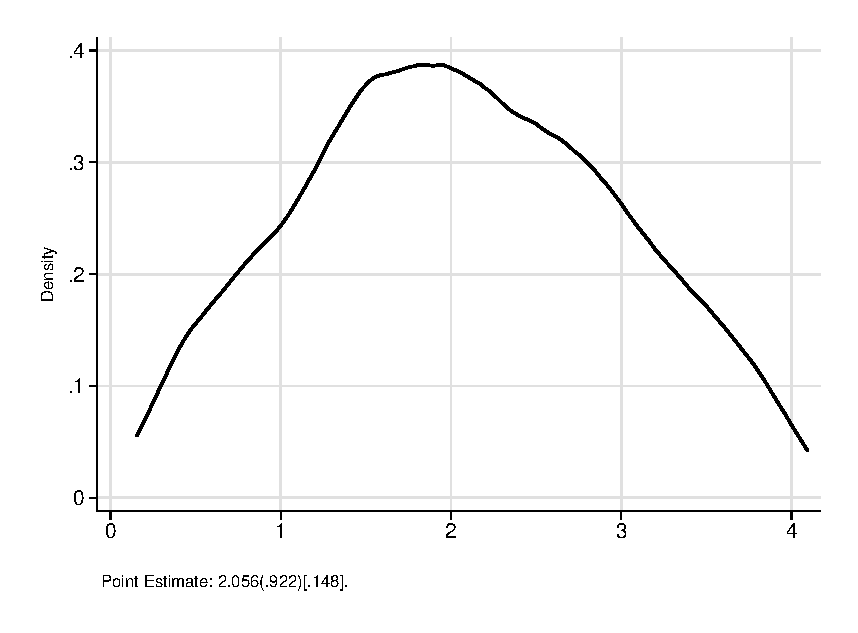
\includegraphics[width=.8\columnwidth]{output/ratios_8_sexf.eps}
\end{figure}
\end{frame}

%% ---------------------------------------------------------------------------

\begin{frame}
\frametitle{B/C Males, Treatment vs. Control (Alternative Preschools)} 
\begin{figure}
	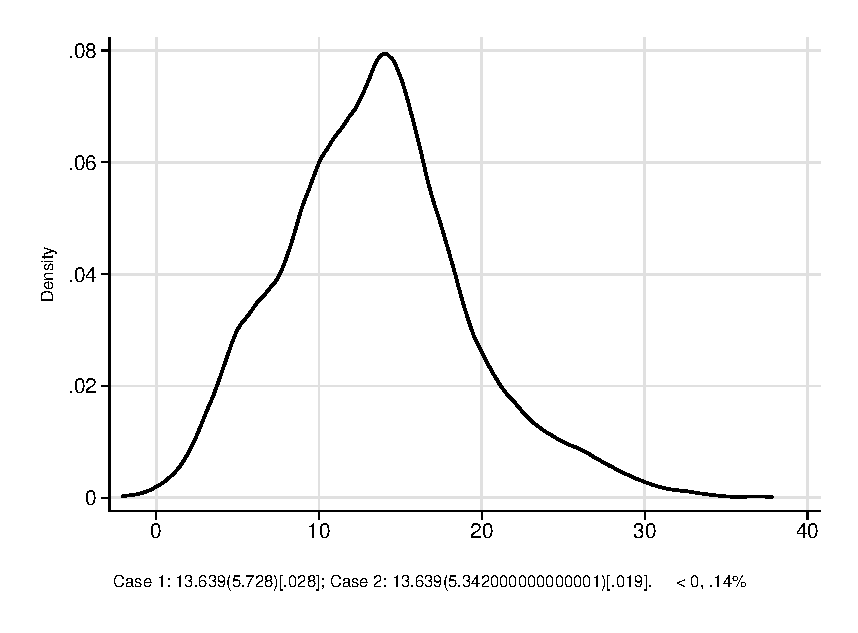
\includegraphics[width=.8\columnwidth]{output/ratios_8_sexm.eps}
\end{figure}
\end{frame}

%% ---------------------------------------------------------------------------

\begin{frame}
\frametitle{B/C Pooled, Treatment vs. Control (Alternative Preschools)} 
\begin{figure}
	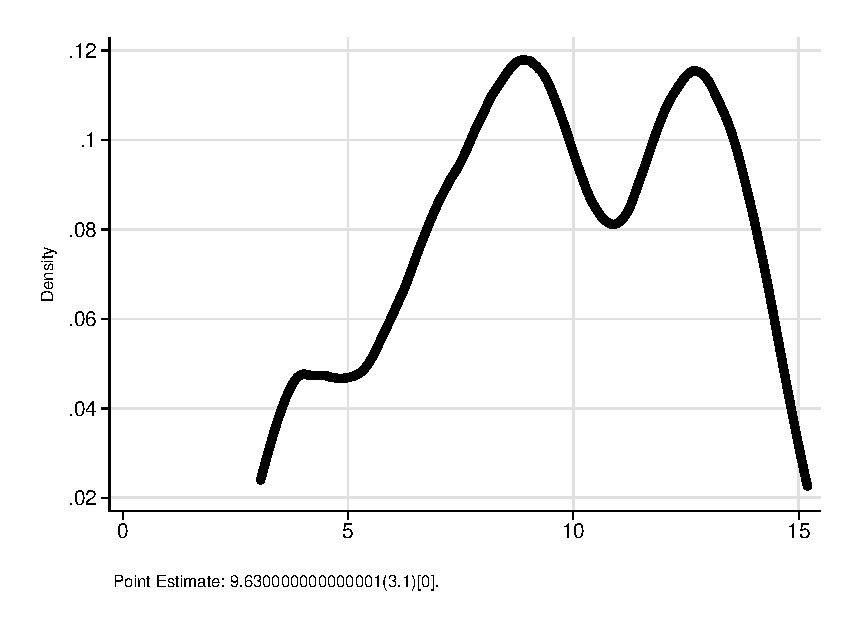
\includegraphics[width=.8\columnwidth]{output/ratios_8_sexp.eps}
\end{figure}
\end{frame}

%% ---------------------------------------------------------------------------

\begin{frame}
\frametitle{Current Estimates}
\begin{center}
\begin{table}
	\caption{CBA Summary}
	\scalebox{.60}{\begin{tabular}{l c c c c c c }
\toprule
	&	\mc{2}{c}{Females}					&	\mc{2}{c}{Males}					&	\mc{2}{c}{Pooled}					\\
		\cmidrule(lr){2-3}						\cmidrule(lr){4-5}						\cmidrule(lr){6-7}					
Estimate 	&	IRR	&	B/C	&	IRR	&	B/C	&	IRR	&	B/C	\\
\midrule

% INSERT summary_tex.xls FILE BELOW
% INSERT summary_tex.xls FILE BELOW
% INSERT summary_tex.xls FILE BELOW

Baseline	&	0.11 	&	3.52	&	\textbf{0.16} &	9.21 	&	\textbf{0.13}	&	\textbf{5.80}	\\
	&	(0.12)	&	(2.67)	&	(0.11)	&	(8.33)	&	(0.06)	&	(2.86)	\\
Relative to Staying at Home	&	-0.14	&	\textbf{4.95}	&	0.06	&	4.29	&	\textbf{0.10} &	5.18	\\
	&	(0.13)	&	(2.02)	&	(0.11)	&	(4.75)	&	(0.05)	&	(3.19)	\\
Relative to Alternative Preschools	&	0.09		&	2.88	&	\textbf{0.21}	&	\textbf{13.64}	&	\textbf{0.13}	&	\textbf{5.56}	\\
	&	(0.11)	&	(1.85)	&	(0.13)	&	(5.72)	&	(0.06)	&	(2.88)	\\

% INSERT summary_tex.xls FILE ABOVE
% INSERT summary_tex.xls FILE ABOVE
% INSERT summary_tex.xls FILE ABOVE

\bottomrule
\end{tabular}}
\end{table}
\end{center}
\end{frame}

%% ---------------------------------------------------------------------------

\begin{frame}
\frametitle{Current Estimates, Trimming}
\begin{center}
\begin{table}
	\caption{CBA Summary}
	\scalebox{.60}{\begin{tabular}{l c c c c c c }
\toprule
	&	\mc{2}{c}{Females}					&	\mc{2}{c}{Males}					&	\mc{2}{c}{Pooled}					\\
		\cmidrule(lr){2-3}						\cmidrule(lr){4-5}						\cmidrule(lr){6-7}					
Estimate 	&	IRR	&	B/C	&	IRR	&	B/C	&	IRR	&	B/C	\\
\midrule

% INSERT summary_tex.xls FILE BELOW
% INSERT summary_tex.xls FILE BELOW
% INSERT summary_tex.xls FILE BELOW

Baseline	&	0.10 	&	\textbf{2.59}	&	\textbf{0.14} &	\textbf{9.75} 	&	\textbf{0.13}	&	\textbf{5.58}	\\
	&	(0.07)	&	(0.97)	&	(0.05)	&	(4.59)	&	(0.05)	&	(2.32)	\\
Relative to Staying at Home	&	\textbf{0.15}	&	\textbf{4.81}	&	\textbf{0.09}	&	4.32	&	\textbf{0.10} &	\textbf{4.42}	\\
	&	(0.07)	&	(1.42)	&	(0.04)	&	(2.70)	&	(0.03)	&	(1.39)	\\
Relative to Alternative Preschools	&	0.10		&	\textbf{2.37}	&	\textbf{0.17}	&	\textbf{12.38}	&	\textbf{0.14}	&	\textbf{6.29}	\\
	&	(0.07)	&	(0.91)	&	(0.05)	&	(5.16)	&	(0.04)	&	(2.23)	\\

% INSERT summary_tex.xls FILE ABOVE
% INSERT summary_tex.xls FILE ABOVE
% INSERT summary_tex.xls FILE ABOVE

\bottomrule
\end{tabular}}
\end{table}
\end{center}
\end{frame}

%% ---------------------------------------------------------------------------

\begin{frame}
\frametitle{Current Estimates, No Controls}
\begin{center}
\begin{table}
	\caption{CBA Summary}
	\scalebox{.60}{\begin{tabular}{l c c c c c c }
\toprule
	&	\mc{2}{c}{Females}					&	\mc{2}{c}{Males}					&	\mc{2}{c}{Pooled}					\\
		\cmidrule(lr){2-3}						\cmidrule(lr){4-5}						\cmidrule(lr){6-7}					
Estimate 	&	IRR	&	B/C	&	IRR	&	B/C	&	IRR	&	B/C	\\
\midrule

% INSERT summary_tex.xls FILE BELOW
% INSERT summary_tex.xls FILE BELOW
% INSERT summary_tex.xls FILE BELOW

Baseline	&	\textbf{0.10} 	&	3.08&	\textbf{0.17} &	\textbf{9.66} 	&	\textbf{0.11}	&	\textbf{4.89}	\\
	&	(0.08)	&	(2.40)	&	(0.11)	&	(5.14)	&	(0.08)	&	(2.83)	\\
Relative to Staying at Home	&	\textbf{0.13}	&	6.64	&	0.05	&	3.11	&	\textbf{0.11} &	6.59 	\\
	&	(0.09)	&	(4.85)	&	(0.13)	&	(4.74)	&	(0.06)	&	(4.69)	\\
Relative to Alternative Preschools	&	0.09		&	1.87	&	\textbf{0.20}	&	\textbf{13.98}	&	0.12	&	4.72	\\
	&	(0.11)	&	(2.21)	&	(0.13)	&	(6.17)	&	(0.10)	&	(3.22)	\\

% INSERT summary_tex.xls FILE ABOVE
% INSERT summary_tex.xls FILE ABOVE
% INSERT summary_tex.xls FILE ABOVE

\bottomrule
\end{tabular}}
\end{table}
\end{center}
\end{frame}

%% ---------------------------------------------------------------------------

\begin{frame}
\frametitle{Current Estimates, Trimming and No Controls}
\begin{center}
\begin{table}
	\caption{CBA Summary}
	\scalebox{.60}{\begin{tabular}{l c c c c c c }
\toprule
	&	\mc{2}{c}{Females}					&	\mc{2}{c}{Males}					&	\mc{2}{c}{Pooled}					\\
		\cmidrule(lr){2-3}						\cmidrule(lr){4-5}						\cmidrule(lr){6-7}					
Estimate 	&	IRR	&	B/C	&	IRR	&	B/C	&	IRR	&	B/C	\\
\midrule

% INSERT summary_tex.xls FILE BELOW
% INSERT summary_tex.xls FILE BELOW
% INSERT summary_tex.xls FILE BELOW

Baseline	&	\textbf{0.10} 	&	3.08&	\textbf{0.17} &	\textbf{9.66} 	&	\textbf{0.11}	&	\textbf{4.89}	\\
	&	(0.06)	&	(2.22)	&	(0.11)	&	(4.72)	&	(0.07)	&	(2.64)	\\
Relative to Staying at Home	&	\textbf{0.13}	&	6.64	&	0.05	&	3.11	&	\textbf{0.11} &	6.59 	\\
	&	(0.09)	&	(4.63)	&	(0.11)	&	(4.46)	&	(0.06)	&	(4.47)	\\
Relative to Alternative Preschools	&	0.09		&	1.87	&	\textbf{0.20}	&	\textbf{13.98}	&	0.12	&	4.72	\\
	&	(0.08)	&	(2.02)	&	(0.13)	&	(5.72)	&	(0.09)	&	(3.04)	\\

% INSERT summary_tex.xls FILE ABOVE
% INSERT summary_tex.xls FILE ABOVE
% INSERT summary_tex.xls FILE ABOVE

\bottomrule
\end{tabular}}
\end{table}
\end{center}
\end{frame}
\clearpage

%% ---------------------------------------------------------------------------
%% ----------------------------Appendix slides-----------------------------------------------

\appendix

%% ---------------------------------------------------------------------------


%%
%%--------------------------- Content ends here ---------------------------------------------------
%%

% --------------------- Bibliography hidden with a save box ---------------------------------------
\mode<all>
\bibliographystyle{chicago}
\savebox\hiddenbib{\parbox{\textwidth}{\bibliography{heckman}}}

\end{document} 